\begin{frame}
    \begin{figure}
        \centering
        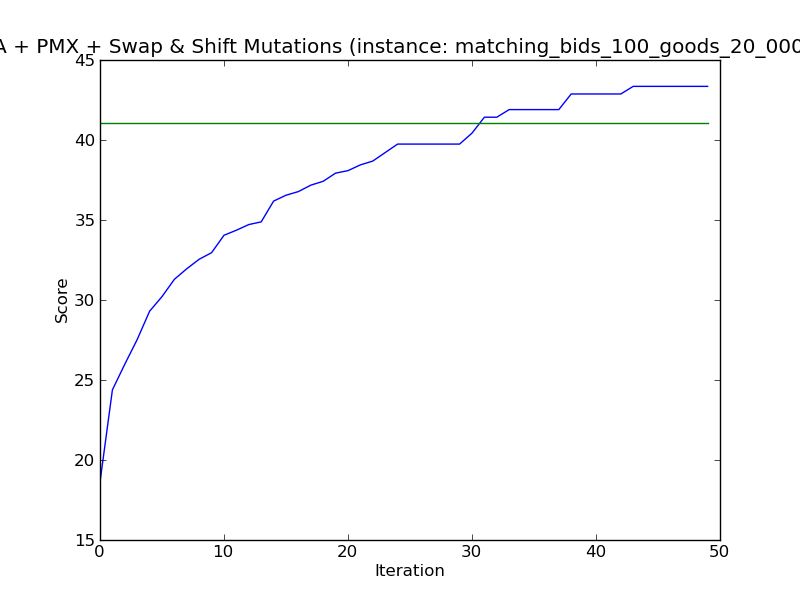
\includegraphics[width=10cm]{wykresy/matching_bids_100_goods_20_0000_txt_1.png}
        \caption{Wykres dla problemu 'matching' o parametrach 20 ofert i 100 towarów.}
    \end{figure}
\end{frame}

\begin{frame}
    \begin{figure}
        \centering
        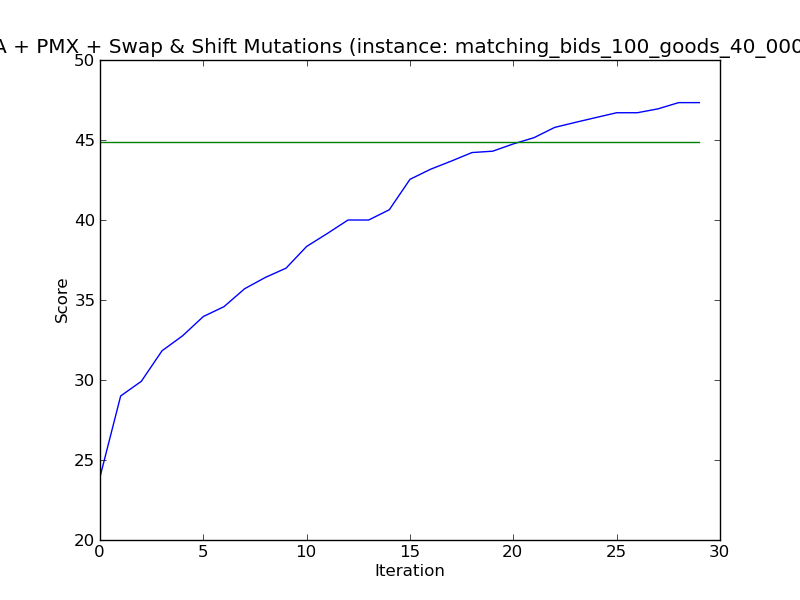
\includegraphics[width=10cm]{wykresy/matching_bids_100_goods_40_0000_txt_3.png}
        \caption{Wykres dla problemu 'matching' o parametrach 40 ofert i 100 towarów.}
    \end{figure}
\end{frame}

\begin{frame}
    \begin{figure}
        \centering
        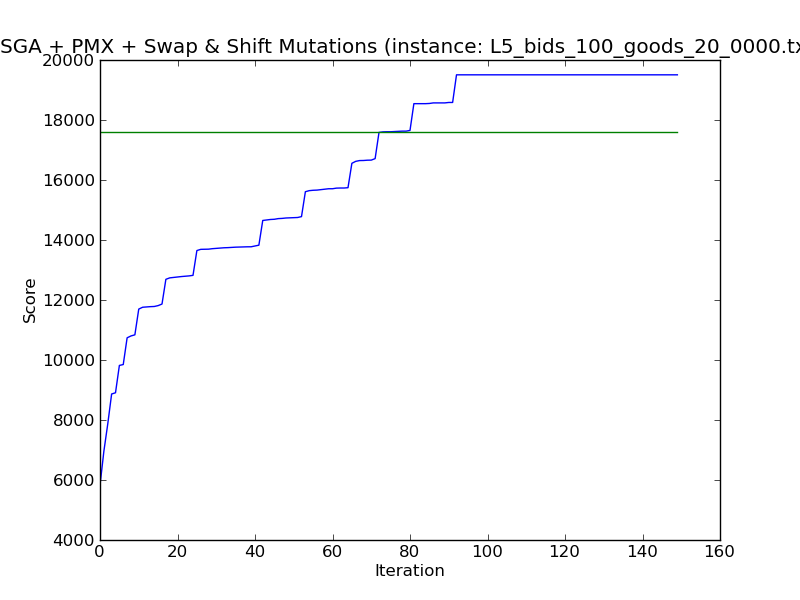
\includegraphics[width=10cm]{wykresy/L5_bids_100_goods_20_0000_txt_1.png}
        \caption{Wykres dla problemu 'L5' o parametrach 20 ofert i 100 towarów.}
    \end{figure}
\end{frame}

\begin{frame}
    \begin{figure}
        \centering
        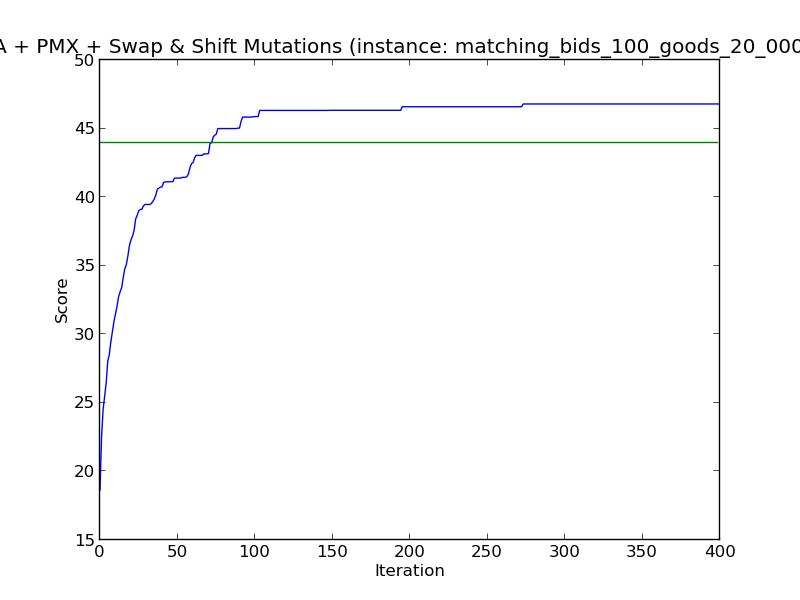
\includegraphics[width=10cm]{wykresy/matching_bids_100_goods_20_0000_txt_uniq.png}
    \end{figure}
\end{frame}

\begin{frame}{Podsumowanie}
\begin{itemize}
\item Rozwiązania PBILa były porównywalne z algorytmem losowym (czyli reprezentacja binarna była nieskuteczna dla tego problemu).
\item Rozwiązania SGA są nieco lepsze niż wyniki algorytmu losowego.
\item Głównym problemem jest bardzo szybka zbieżność populacji (przy czym dotyczy to wartości funkcji celu, a nie różnorodności samych osobników).
\item Reprezentacja permutacja też nie jest idealna (duża część permutacji nie wpływa na faktyczne rozwiązanie, operatory genetyczne muszą być odpowiednio dostosowane).
\end{itemize}
\end{frame}
